\documentclass{article}
\usepackage[utf8]{inputenc}

\usepackage{natbib}
\usepackage{graphicx}

\title{Visualization and Interpretability}
\author{yusuf.roohani@gmail.com}
\date{August 2017}

\begin{document}
\maketitle

\section{Dimensionality reduction}

These are notes made during a talk by Laurens van der Maaten at Google in 2013 \cite{vdMaaten}

\subsection{PCA}

    Linear projection of the data, such that the variance between data points is maximized. Tries to make sure that stuff that is dissimilar ends up far apart, so it's better at preserving large pariwise distances
    
\subsection{Locally linear embedding}
    Attempts to preserve small pairwise distances but tends to cluster all points at the origin
    
\subsection{t-dsitibuted Stochastic Neighbor Embedding (tSNE)}
    A non-linear dimensionality reduction that also preserves small pairwise distances such that similar objects are modeled by similar points and dissimlar objects are modeled by distant points. 
    
    Work with two distributions $p_{i,j}$ in the high-dimensional space and ${q_{i,j}$ in the low-dimensional space, where $i,j$ are data points. For any given point in the high dimensional space, center a gaussian at that point and measure the density of all other points under this Gaussian. Repeat for all points and then renormalize
    
    $$ Missing_equation $$
    
    This gives the similarity between paris of points $i,j$. In practice, conditional probability is computed instead of calculating the joint probability directly. Then, repeat this procedure in low dimensional space, but use a t-distribution for $q_{i,j}$ instead of a Gaussian. 
    
    $$ Missing_equation $$
    
    Now, the goal is to make $q_{i,j}$ represent $p_{i,j}$ as much as possible. So, we use KL divergence to measure the distance between the two probability distributions
    
    \subsection{Why does this work?}
    
    If you have a high value of $p_{i,j}$, then you must make sure that you have a high value of $q_{i,j}$ otherwise you'll have a high penalty, as described by the definition of KL divergence
    
    $$ missing_equation$$
    
    On the other hand, if small $p_{i,j}$ is modeled by large $q_{i,j}$ then the penalty is not as large. Thus, tSNE really emphasizes the local structure of the data.
    
    Also, the reason we use a t distribution instead of Gaussian is because as we go down to lower dimensions, our preference for small scale similarity often causes dissimilar points to be modeled too far apart. The fat tails on a t-distribution allow for that.

\section{Model Interpretability}

Need to read this still \cite{zeiler2014visualizing}

\subsection{Image saliency maps}

Given an image $I_o$, a class $c$ and a classification convnet with a class score function of $S_c(I)$, image specific class saliency maps attempt to rank the pixels of $I_o$ by their influence on the score $S_c(I_o)$ \cite{simonyan2013deep}

We know that the linear score for an image $I$ can be represented as,

$$ S_c(I) = w_c^T*I + b_c $$

From this, it is clear that the magnitude of the elements of w define the importance of the corresponding pixels. However, $S_c$ is a highly nonlinear function. Given an image $I_o$, we can approximate the value of $S_c(I)$ with a linear function in the neighborhood of $I_o$ by using the first-order Taylor series expansion:

$$ S_c(I) \approx w^T I + b$$ 

where $w$ is the derivative 

$$ w = \frac{\partial S_c}{\partial I} $$

One way to think about this is - which pixels need to be changed the least to change the class score the most

\subsubsection{Extracting saliency maps}

\begin{figure}[h!]
\centering
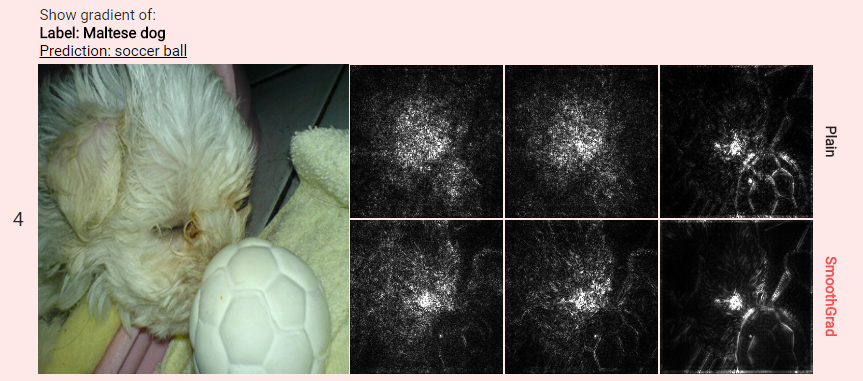
\includegraphics[scale=0.6]{Saliency_catch_mispredict.PNG}
\caption{Saliency maps being used to understand the source of a misprediction}
\label{fig:saliency}
\end{figure}

\begin{itemize}
    \item First the derivative is found by backpropogation
    \item Saliency map is obtained by rearranging elements in the vector $w$. In case of a single channel, this is straightforward, in case of three channels we take the maximum across the channels for each pixel
    \item 
\end{itemize}

\bibliographystyle{plain}
\bibliography{references}

\end{document}